\section{The endpoint field and a four-arm estimate}
\label{sec:q4tools}

Throughout this section and the next, $q=4$ and $p=p_c=2/3$.
We use the critical isotropic square-lattice law, with mesh $\delta$.
The medial loop weight is $2$.  Resolve each contact inside a disk of
radius less than $\delta/100$, preserving the prescribed pairing, so
that the lattice loops are disjoint simple curves.  These resolutions
change uniform curve distance by $O(\delta)$ and do not cross an actual
open primal or dual edge.  Orient each strand by the convention that
primal vertices lie on its left.  Independently for each loop, choose
with equal probabilities this orientation or its reverse.  The resulting
height has jumps of size one.  In the plane it is defined modulo a
constant; its pairing with a smooth compactly supported density of
integral zero is well defined.

We fix the normalization
\begin{equation}\label{q4field:normalization}
 G_{\mathbb C}(x,y)=-\frac{1}{2\pi}\log|x-y|,
 \qquad \sigma^2=\frac{2}{\pi},
 \qquad \lambda_0=\sqrt{\frac{\pi}{8}},
 \qquad 2\sigma\lambda_0=1.
\end{equation}
Thus $\Phi_V$ will denote the Dirichlet free field whose covariance is
the Green operator for $-\Delta$ on $V$.

\begin{lemma}[Comparison of height conventions]\label{q4field:height-comparison}
Couple the cellwise lattice height $h_\delta^{\mathrm{cell}}$ and
the height $h_\delta^{\mathrm{geom}}$ defined by the smoothed loop
interiors using the same independent loop signs.  For every smooth
compactly supported neutral density $\rho$,
\begin{equation}\label{q4field:height-comparison-L2}
 \mathbb E\left|
   \langle h_\delta^{\mathrm{geom}}
          -h_\delta^{\mathrm{cell}},\rho\rangle\right|^2
 \longrightarrow0.
\end{equation}
This conclusion uses only bulk crossing and passage-count estimates.
\end{lemma}

\begin{proof}
Decompose $\rho$ into a finite linear combination of differences of
smooth unit masses.  For a single such difference, sample its two
endpoints independently at each of the two occurrences in the second
moment.  For a loop $L$, let $d_i^{\mathrm{geom}}(L)$ and
$d_i^{\mathrm{cell}}(L)$ be its winding-indicator differences for
the two height conventions at the $i$-th endpoint pair.  Averaging
the common fair signs gives the mixed second-moment integrand
\[
 \mathbb E\sum_L
   \bigl(d_1^{\mathrm{geom}}(L)-d_1^{\mathrm{cell}}(L)\bigr)
   \bigl(d_2^{\mathrm{geom}}(L)-d_2^{\mathrm{cell}}(L)\bigr).
\]
At a fixed tuple of four distinct endpoints, put $d_*>0$ for their
minimum separation, truncated at one.  A nonzero term requires the
same loop to enter an $O(\delta)$ neighborhood of an endpoint of
each pair.  For small enough $\delta$ that loop has diameter at
least $d_*/2$.  The bulk one-arm estimate makes such a macroscopic
loop's approach to a mesh-sized endpoint neighborhood negligible.
Higher passage-count moments give uniform integrability on each
fixed size range; the arm bound for a loop visiting the bounded
support and reaching a large radius removes the remaining tail.
Thus this integrand tends to zero at every distinct endpoint tuple.

The octave passage-count bounds also give the integrable majorant
$C(1+|\log(d_*\vee\delta)|)^2$.  Indeed every contributing loop has
size at least the endpoint separation up to a mesh error, the count
has bounded moments per octave, and the outer octaves have a
power-decaying tail.  The same estimate holds for each of the four
mixed terms in the displayed product.  Dominated convergence in
the independently sampled endpoints proves
\eqref{q4field:height-comparison-L2}; tuples with coincidences have
zero integration measure.  A finite linear decomposition and
Cauchy--Schwarz give the assertion for $\rho$.
\end{proof}

\begin{proposition}[Whole-plane height convergence]\label{q4field:wholeplane-input}
For every real $\rho\in C_c^\infty(\mathbb C)$ with $\int\rho=0$,
the independent fair unit-jump height of critical square-lattice
$\FK_4$ satisfies
\begin{equation}\label{q4field:plane-characteristic}
 \lim_{\delta\downarrow0}
 \mathbb E\exp\bigl(i\langle h_\delta,\rho\rangle\bigr)
 =\exp\left\{-\frac{\sigma^2}{2}
  \iint\rho(x)G_{\mathbb C}(x,y)\rho(y)\,dx\,dy\right\}.
\end{equation}
The same assertion holds jointly for finitely many such tests.
\end{proposition}

\begin{proof}
Corollary~\ref{cor:rr-gff-input} gives this statement for the cellwise
height.  Lemma~\ref{q4field:height-comparison} transfers it to the
smoothed geometric height, since the difference of the characteristic
functions is bounded by
$\mathbb E|\langle h_\delta^{\mathrm{geom}}
-h_\delta^{\mathrm{cell}},\rho\rangle|$.  Apply the same argument
to every real linear combination of finitely many tests to obtain
joint convergence.
\end{proof}

The parameters in \citet[Theorem~2.8 and Corollary~3.2]{SixVertexGFF2026}
are $c=2$, $\Delta=-1$, and $\mu=0$.  The loop factor is then an
ordinary cosine, exactly the characteristic function of a fair sign
multiplying a unit jump.  The proposition concerns only the
whole-plane field; finite-domain and conditional-field statements
are proved below.

\subsection{Moments and binary transport}

We first record why characteristic-function convergence supplies the
moments used below.  This argument uses only the bulk crossing theorem,
which includes $q=4$ \citep{DCLM2019Isoradial}, and the actual-component
counting argument of Section~\ref{sec:preliminaries}.

\begin{lemma}[Neutral moment bounds]\label{q4field:neutral-moments}
For finitely many smooth compactly supported neutral densities, their
height pairings have uniformly bounded moments of every fixed order.
All their joint moments converge to the corresponding Gaussian
moments.  The bounds and limits
are unchanged by the $O(\delta)$ drawing modifications just described.
\end{lemma}

\begin{proof}
It suffices, by linear decomposition, to use differences of two smooth
unit masses.  Expand a product of $m$ such pairings, integrating the two
endpoints of each occurrence separately.  For fixed sampled endpoints
$a_i,b_i$, put
\[
 d_i(L)=\mathbf1_{\{a_i\in\operatorname{int}L\}}
       -\mathbf1_{\{b_i\in\operatorname{int}L\}}.
\]
Conditional on the loops, averaging the fair signs gives exactly
\begin{equation}\label{q4field:even-assignment}
 \mathbb E_{\epsilon}\prod_{i=1}^m
       \sum_L\epsilon_Ld_i(L)
 =\sum_{f:\{1,\ldots,m\}\to\{\text{loops}\}}
       \prod_i d_i(f(i))
       \prod_L\mathbf1_{\{|f^{-1}(L)|\text{ is even}\}}.
\end{equation}
In a nonzero term every used loop separates the endpoints in each slot
assigned to it and is used in at least two slots.  If $d_*$ is the
smallest distance between the $2m$ sampled endpoints, truncated at $1$,
such a loop has diameter at least $d_*$.  Notice that even repeated
copies of the same smeared charge have separately sampled endpoints;
coincidences have zero integration measure.

For each endpoint and each size octave, the number of loops of that
size which wind around it has moments of every order bounded uniformly
in the mesh.  Indeed such a loop supplies a passage in one of a bounded
number of buffered annuli of comparable size.  Ordering their medial
passages produces distinct actual bank components, with bounded
multiplicity.  Successive actual-component exploration and bulk RSW
give a geometric tail for this count.  Between $d_*$ and the diameter
of the fixed support there are $O(1+|\log d_*|)$ octaves.  For larger
loops, separation of two support points forces a visit to a fixed
bounded slit joining them.  Reaching the octave of radius $R$ then
requires an actual arm from that bounded region to scale $R$, whose
probability decays as a power of $R$.  Cauchy--Schwarz and higher
passage-count moments make the sum of these outer octaves finite.
Consequently the absolute value of the integrand in
\eqref{q4field:even-assignment}, after expectation, is bounded by
\[
 C_m\bigl(1+|\log(d_*\vee\delta)|\bigr)^m.
\]
The same reasoning bounds any fixed higher absolute moment of the
geometric majorant.  Logarithmic singularities are locally integrable
in the independently sampled endpoints.  This proves uniform
integrability of every fixed moment.  Proposition~\ref{q4field:wholeplane-input}
and uniform integrability now give joint moment convergence.

If a drawing modification changes a contributing indicator at one of
a fixed collection of distinct sampled endpoints, a loop of positive
diameter enters an $O(\delta)$ neighborhood of that endpoint.  The
bulk one-arm estimate makes this event negligible; the preceding
higher moment bounds allow its removal under the integrals.
\end{proof}

The binary index propagates by equality along every directed strand.
At a tile, sum the two possible pairings with equal coefficient.
An inserted matrix acts on this binary index, and a closed loop with
ordered insertions $M_1,\ldots,M_k$ has conditional response
$\tfrac12\operatorname{tr}(M_1\cdots M_k)$.  Thus the unperturbed loop
weight is $\operatorname{tr}I=2$.

\begin{lemma}[The reflected vacuum]\label{q4field:reflection}
The plane binary-index network is reflection positive across the
translated lattice symmetry lines parallel to either axis or to a
diagonal.  Reflection reverses directed transport and takes inserted
matrices to their adjoints.  Simultaneous conjugation by $SU(2)$ is
unitary on the reflected Hilbert space.
\end{lemma}

\begin{proof}
For a vertical cut through a primal column, a bisected tile contributes
the seam operator
\[
 I+|\mathrm{Bell}\rangle\langle\mathrm{Bell}|,
 \qquad \mathrm{Bell}=e_1\otimes e_1+e_2\otimes e_2,
\]
which is positive.  The horizontal case is identical.  A diagonal cut
along tile edges contracts equal indices, and is positive as well.
These statements give a positive Gram form for arbitrary finite
network replacements strictly on one side of the cut.  Each switch
intertwines the transports on its reference-directed pairs, so
simultaneous conjugation preserves all contractions; reflection
therefore implements it unitarily.

One may first use large reflection-periodic tori, with two reflection
seams.  For a diagonal seam take periods along and perpendicular to the
diagonal.  The all-loop torus measure differs from periodic FK by a
bounded genus factor.  A fixed patch is, with probability tending to
one, screened by contractible actual circuits of both colors.  On that
event the genus data are exterior to the patch.  Bulk uniqueness and
the circuit tails identify every local subsequential limit with the
plane FK state.  Equivalently, finite closure of all strands meeting
the patch gives its plane domain Markov law directly.  Independent
binary indices pass to this limit.  The finite-volume positive forms
therefore give the asserted plane form.
\end{proof}

\subsection{From the spin-two sector to four arms}

Write $\pi_4^\delta(r,R)$ for the plane probability of four alternating
actual primal and dual arms across a square annulus.  Fixed changes of
its rims change this probability by at most constant factors.  We use
also separated prescribed landing sectors and their buffered
extensions, at a bounded multiplicative cost.  These are bulk
statements at $p_c$; the published alternating-arm result includes
$q=4$ \citep[Proposition~2.3 and the arm-separation discussion]{DM2022Scaling}.
No boundary RSW theorem at $q=4$ is used.

\begin{proposition}[A bulk four-arm bound]\label{q4field:four-arm}
There is a constant $C$ such
that, for $0<r<R$,
\begin{equation}\label{q4field:four-arm-bound}
 \limsup_{\delta\downarrow0}\pi_4^\delta(r,R)
 \le C(r/R)^2.
\end{equation}
The same bound, with a constant depending on the fixed bulk collar,
holds inside a domain with arbitrary exterior boundary data.
\end{proposition}

\begin{proof}
Scale the outer radius to a fixed small constant.  Choose mirror boxes
of radius $s$ at horizontal distance one, centered at $x$ and $y$.
In the box at $x$, take a positive unit mass in a disk of radius
$\varepsilon s$ at $x+(s/2,0)$ and a negative unit mass near
$x-(s/2,0)$; use their reflected placement at $y$.  Fix smooth mass
profiles and connecting slits inside the boxes.  Their height
differences are denoted $h_x,h_y$.

For a traceless complex $2\times2$ matrix $V$, insert
$\exp(taV)$ along each successive directed flux piece, where $a$ is
its contribution to this smeared dipole.  Equivalently, if $\rho_x$
is the dipole density, choose a compactly supported one-form
$\alpha_x$ in its box with $d\alpha_x=\rho_x\,dx\wedge dy$,
and integrate $\alpha_x$ along the directed pieces.  Such a form
exists because $\int\rho_x=0$.  Let $A(V)$ be the
second-order coefficient as a vector in the reflected space.  It is
an equivariant quadratic map on the complexified conjugation
representation of $SU(2)$.  Its symmetric square decomposes into a
scalar representation and one irreducible spin-two representation.
Set
\[
 E=e_1e_2^*,\qquad F=E^*,\qquad H=\operatorname{diag}(1,-1).
\]
The tensor $E\otimes E$ lies entirely in spin two, whereas the
spin-two projection of $H\otimes H$ is nonzero.  Unitary equivariance
and irreducibility therefore give, with an absolute constant,
\begin{equation}\label{q4field:spin-two}
 \|A(E)\|^2
 \le C\left\|A(H)-\frac12\mathbb E(h_x^2)\mathbf1\right\|^2
 =\frac C4\operatorname{Cov}(h_x^2,h_y^2).
\end{equation}
Here $\mathbf1$ is the vacuum vector.  This does not assert that the
entire scalar sector consists of multiples of $\mathbf1$: projection
onto spin two annihilates $\mathbf1$, which is all the inequality
requires.  For diagonal $H$, the second coefficient is $h_x^2/2$,
giving the last equality with the reflected orientation convention.

By Lemma~\ref{q4field:neutral-moments}, the covariance in
\eqref{q4field:spin-two} converges to its Gaussian value.  The covariance
of the two neutral charges is $O(s^2)$, since the logarithmic kernel
is smooth between the boxes and each charge has total mass zero and
first absolute moment $O(s)$.  The Gaussian identity
$\operatorname{Cov}(X^2,Y^2)=2\operatorname{Cov}(X,Y)^2$ gives
\begin{equation}\label{q4field:spin-upper}
 \limsup_{\delta\downarrow0}\|A(E)\|^2\le C_\varepsilon s^4.
\end{equation}

We obtain a matching lower bound from two passages at each box.
For a loop visiting both boxes, compress each maximal run at one box
before its next visit to the other into one factor.  Nilpotence gives
alternating factors
\[
 I+ta_1E,\ I+ub_1F,\ I+ta_2E,\ I+ub_2F,\ldots.
\]
Close an excursion by an arc through the omitted other box,
where the relevant one-form vanishes.  The closing arc can be chosen
disjoint from the excursion, giving a simple curve.  Its flux is an
averaged winding difference, so $|a_i|,|b_i|
\le1$.  The fluxes are integers if the excursions avoid the endpoint
supports.  Let $M$ be the total number of alternating periods, over
all loops visiting both boxes.  There are $2M$ disjoint connecting
passages.  The coefficient $K$ of $t^2u^2$ in the product of normalized
traces satisfies
\begin{equation}\label{q4field:coefficient-bound}
 |K|\le C M^4,\qquad K=0\quad\hbox{if }M<2.
\end{equation}
Loops visiting only one box contribute $1$ and can be omitted.

If $M=2$ and the endpoint supports are missed, then $K\ge0$.
For a single two-period loop its only possible nonzero contribution is
$a_1a_2b_1b_2/2$.  The full winding difference belongs to
$\{-1,0,1\}$, so nonzero integer fluxes satisfy
$a_1=-a_2$ and $b_1=-b_2$; the coefficient is $1/2$.
For two one-period loops the coefficient is
$a_1b_1a_2b_2/4$.  If nonzero, both simple loops separate the two
endpoint pairs.  Their interiors are disjoint or nested, so their
choices of the contained endpoints either agree in both boxes or are
complementary in both.  Hence the products $a_1b_1$ and $a_2b_2$ have
the same sign, and this coefficient is $1/4$.

For completeness, the errors in this sign calculation must be
\emph{relative} to two four-arm probabilities.  Let
$\pi_4=\pi_4^\delta(c_1s,c_2)$, for fixed suitable constants.  Bulk
component searches give
\begin{align}
 \mathbb E\bigl[M^4\mathbf1_{\{M\ge3\}}\bigr]
   &\le o_s(1)\pi_4^2,\label{q4field:relative-tail}\\
 \mathbb P(M=2,\text{ an endpoint support is hit})
   &\le C\varepsilon^\alpha\pi_4^2,\label{q4field:relative-hit}
\end{align}
for some $\alpha>0$, with the mesh taken sufficiently small at each
fixed $s,\varepsilon$.  Here is the exploration underlying these
estimates.  Around either box the $2M$ radial separators, cropped with
end margins, give $2M$ alternating bank arms and at least $M$ distinct
actual primal crossing components of a cropped annulus.  Conversely,
two distinct actual primal crossing components force two intervening
dual separators, hence four alternating arms in a slightly narrower
annulus.  Thus the first two successful discoveries already cost
$C\pi_4$.  Expose each complete actual component, including all its
exiting edges revealed closed, and do not count wire identifications
as open paths.  The remaining graph is dominated by
the original annular lattice with maximal identifications at its
original rims.  In separated dyadic rings, a buffered dual circuit
blocks every actual radial crossing with uniformly positive
conditional probability.  Each further discovered crossing therefore
costs at most $Cs^\alpha$.  Iterating this bound gives a summable tail
even after multiplication by $M^4$.  The two box annuli have disjoint
bulk collars, so their first-four-arm costs multiply up to a constant;
this proves \eqref{q4field:relative-tail}.  An endpoint hit additionally
requires a bank arm from radius $\varepsilon s$ to a fixed small
multiple of $s$, in a buffered region inside the hole of its
corresponding four-arm annulus.  Both four-arm costs are retained.
The same conditional blocking estimate proves
\eqref{q4field:relative-hit}.  In particular an absolute $o(1)$ bound
would not suffice in either estimate.

Finally there is a compatible positive event of probability at least
$c\pi_4^2$, with $c$ independent of sufficiently small $\varepsilon$.
Prescribe primal east/west and dual north/south landings
at each box annulus, with buffered extensions.  Attach the two primal
inner landings to small actual circuits around the positive and
negative endpoint disks, respectively, at radii $\eta s$,
where the small constant $\eta>0$ is fixed before choosing
$\varepsilon\ll\eta$.  At the large scale join the inward primal arms
directly between the boxes, and the outward pair around their
exterior.  Join the upper dual arms to each other and the lower dual
arms to each other between these routes.  At each inner rim join its
two dual arms in a central corridor between the terminals.  Together
these dual connections form a closed oval separating the two primal
groups.  Retain one inner-to-outer landing pairing of comparable
probability at the first annulus and its mirror at the second; the
gluing works for either pairing.  One of the two pairing classes
has at least half the separated-arm probability, so no additional
theorem concerning a prescribed pairing is needed.

\begin{figure}[tbp]
\centering
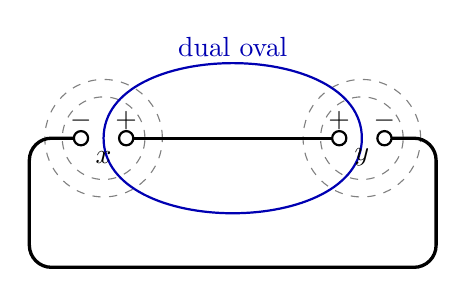
\begin{tikzpicture}[scale=.82]
 \draw[gray,dashed] (-2,0) circle (.64);
 \draw[gray,dashed] (-2,0) circle (.91);
 \draw[gray,dashed] (2,0) circle (.64);
 \draw[gray,dashed] (2,0) circle (.91);
 \draw[very thick] (-1.65,0)--(1.65,0);
 \draw[very thick,rounded corners=8pt]
   (-2.35,0)--(-3.15,0)--(-3.15,-2)--(3.15,-2)--(3.15,0)--(2.35,0);
 \draw[blue!70!black,thick]
   (-2,0) .. controls (-2,1.55) and (2,1.55) .. (2,0)
          .. controls (2,-1.55) and (-2,-1.55) .. cycle;
 \foreach \x in {-2.35,-1.65,1.65,2.35}
   {\draw[thick,fill=white] (\x,0) circle (.11);}
 \node at (-1.65,.28) {$+$};
 \node at (1.65,.28) {$+$};
 \node at (-2.35,.28) {$-$};
 \node at (2.35,.28) {$-$};
 \node at (-2,-.3) {$x$};
 \node at (2,-.3) {$y$};
 \node[blue!70!black] at (0,1.42) {dual oval};
\end{tikzpicture}
\caption{The bulk gluing used in the lower bound.  Black connections
join the positive terminals and the negative terminals separately;
the dual oval keeps these two actual primal clusters distinct.
Each terminal is protected by a small primal circuit.  Only
connectivity is depicted; the four-arm annuli are schematic.}
\label{q4field:gluing-figure}
\end{figure}

All these joins can be made in finitely many disjoint tubes of the
requested colors, outside the core annuli except for their landing
extensions.  Use transverse crossings in overlap rectangles to join
the extensions to the tubes.  Condition on the complement of one
color's tubes and apply FKG and buffered RSW there, then do the other
color.  Since only that color's extensions enter its tubes, the
requirements are increasing in the appropriate conditional model.
The two core annulus probabilities multiply by the bulk collar
comparison.  The resulting positive and negative terminal circuits
belong to two distinct actual primal clusters, the first connecting
the two positive terminals and the second the two negative ones.

There are at least two distinct closed interfaces separating these
two connected primal groups: color parity makes their number even,
and at least one is necessary.  Each such interface separates both
endpoint pairs and misses their support disks.  On the part of this
event with $M=2$, the two-loop coefficient is $1/4$.  Subtracting
\eqref{q4field:relative-tail} and \eqref{q4field:relative-hit}, first
choose $\varepsilon>0$ small and fixed, and then $s$ small.  Positivity
on all the remaining $M=2$ configurations and
\eqref{q4field:coefficient-bound} show
\[
 \|A(E)\|^2=\mathbb E K\ge c'\pi_4^2.
\]
Combining this with \eqref{q4field:spin-upper} proves
$\limsup_{\delta\downarrow0}\pi_4\le Cs^2$.
Quasi-multiplicativity and fixed-factor rim changes give
\eqref{q4field:four-arm-bound}.  Bulk collars give its domain version.
\end{proof}

\begin{corollary}[Macroscopic contacts]\label{q4field:contact-dimension}
In any tight subsequential
limit of actual loops or Dobrushin strands, the interior set of
genuinely distinct visits by macroscopic curves has Hausdorff dimension
at most zero, almost surely.  Constant parametrization pauses are
discarded.  No assertion about boundary contacts is made here.
\end{corollary}

\begin{proof}
Fix an interior compact set and an outer displacement cutoff $R>0$.
A point with two genuinely distinct visits, each having displacement
at least $R$, gives four medial passages across every sufficiently
small surrounding annulus.  With rim margins, their actual banks
give four alternating arms.  A grid cover at scale $r$ has
$O(r^{-2})$ cells, each with limiting probability at most $C(r/R)^2$.
Its expected number of required cells is therefore bounded uniformly
in $r$, after the mesh limit.  For every $\eta>0$ the expected
$\eta$-dimensional covering content is $O(r^\eta)$; along dyadic
scales it tends to zero almost surely.  Countable compact sets,
displacement cutoffs, and positive $\eta$ prove the claim.
\end{proof}

\section{The field in regular domains}
\label{sec:q4regular}

We now derive the finite-domain statement required for the loop
identification.  It is not part of
Proposition~\ref{q4field:wholeplane-input}.

\subsection{Actual walls and elementary bounds}

Write $C\in\{\mathsf P,\mathsf D\}$ for a color and $C'$ for the other.
An actual homogeneous wall is a simple polygon of $C$-diagonals,
whose switches are forced open in color $C$.  A mixed wall consists
of an actual primal-diagonal arc, an actual dual-diagonal arc, and two
tile sides joining their ends.  Each tile side is a one-port
transition gate.  All interior switches not on a wall are sampled,
including a switch whose diagonal endpoints happen both to lie on
the wall.

\begin{lemma}[Vacuum realization of a wall]\label{q4field:wall-law}
Conditioning the plane vacuum on exactly the stated wall switches
gives the FK law inside with the indicated actual connections.
For a closed $C$-wall, the $C'$ model on the strictly internal sites
and its internal edges has free boundary condition.
In a mixed wall, fixing the binary index at one transition port fixes
the index of the distinguished strand; this condition has probability
$1/2$ conditional on every switch configuration.
\end{lemma}

\begin{proof}
An exterior connection of either color can enter only through the
same-color wall arc, already connected by actual open edges.  Hence
it creates no additional interior partition.  For a closed wall no
$C'$ vertex is wired through that wall, giving the stated free model
(equivalently, apply planar duality).  There are exactly two transition
ports in the mixed experiment.  The loop through one must leave the
interior through the other; its one independent fair index is fixed
by the condition at the first port.
\end{proof}

Set the height to zero on a homogeneous wall.  In a mixed wall, take
height zero on its primal arc and choose the distinguished index so
that its dual arc has height one.  Conditional on the geometry,
\begin{equation}\label{q4field:domain-height}
 h_\delta(z)=u_{*,\delta}(z)
      +\sum_{L\text{ internal}}\epsilon_L
                    \mathbf1_{\{z\in\operatorname{int}L\}},
\end{equation}
where the signs are independent and fair.  In the homogeneous case
$u_{*,\delta}=0$; in the mixed case it is the $0/1$ side function of
the distinguished strand.  Values on the drawn curves are immaterial
in integrals.  For $f\in C_c^\infty$ in the interior, the pairing
$\langle h_\delta,-\Delta f\rangle$ depends only on switches and
binary indices near the support of $f$: integration by parts writes
it as oriented flux against a compactly supported smooth one-form.
It consequently does not depend on the relative height constant.

\begin{lemma}[Free-bank estimates]\label{q4field:free-bank}
Consider a patch in which the bank color $C'$ has no forced open edge
and no boundary identification on any domain wall meeting the patch.
The graph may omit sites or edges.  Counts of disjoint medial
passages between buffered annular rims have moments of every order,
uniformly in the mesh and in the remaining exterior data.  The
probability of an actual $C'$ arm across a ratio $R/r$ is at most
$C_0(r/R)^\beta$ for some $\beta>0$.  These statements hold as well
for a product of free $C'$ models on disjoint subgraphs.  In a bulk
patch either color may be used.
\end{lemma}

\begin{proof}
Order the medial radial separators and crop their actual $C'$ bank
paths with margins at both ends.  Different strips cannot communicate
across a separator, and each strip is charged at most twice.  Thus
many passages force a proportional number of distinct actual
crossing components of the cropped graph.  Reveal these components
successively from one rim, ignoring partition jumps.  A deleted
component does not wire surviving interior sites through its former
neighbors.  Since the wall is free for this color, the remaining
graph is dominated by the full annular lattice with maximal ties
only at its original rims.  A buffered circuit of the other color
blocks actual crossing, with conditional probability bounded below
by bulk RSW.  Iteration gives a geometric tail for the component
count and hence all its polynomial moments.  Applying these blockers
in separated dyadic rings proves the power bound for one arm.
Missing edges or sites only lower actual connectivity; the same
comparison applies to a product on disjoint subgraphs.  Enlarge
inner radii by a fixed mesh multiple whenever needed.
\end{proof}

Take now a fixed simple rectilinear polygon $V$, with two distinct
marked transition points on interiors of straight sides in the mixed
case.  Approximate it by the corresponding actual diagonal walls
within $O(\delta)$, in marked boundary order.  Such approximations
exist: round each color arc on its own lattice and adjust its ends
by $O(\delta)$ to join the two colors by a single tile side at each
transition.  This class of regular domains will suffice for the
later comparison argument.

\begin{lemma}[Moment kernels and compactness]\label{q4field:moment-kernels}
For the regular polygons just specified, the height moment kernels at
distinct interior points $z_1,\ldots,z_m$ satisfy
\begin{equation}\label{q4field:log-kernel}
 \left|\mathbb E\prod_{i=1}^m h_\delta(z_i)\right|
 \le C_m\bigl(1+|\log(d_*\vee\delta)|\bigr)^m,
 \qquad d_*=1\wedge\min_{i<j}|z_i-z_j|,
\end{equation}
with $d_*=1$ when $m=1$.  Here $C_m$ depends on $V$ and $m$,
uniformly over the interior tuples, including those approaching
the boundary.  Geometric majorants for the conditional
signed expansions have higher polynomial moments with corresponding
logarithmic bounds.  Integrated moments are uniformly integrable;
the height laws are tight as local distributions, and their moment
kernels are asymptotically equicontinuous on compact sets of distinct
interior tuples.  The count bounds hold also for arbitrarily shaped
homogeneous walls in a fixed bounded box and for products of disks
of one wall color.
\end{lemma}

\begin{proof}
A loop winding around $z$ and of diameter in $[r,2r]$ lies within
$O(r)$ of $z$ and supplies a macroscopic passage in one of a bounded
number of annuli of radius comparable with $r$.  For a homogeneous
wall use its free bank color.  In a fixed mixed polygon, choose a
subpassage away from the transition points by a fixed fraction of
$r$.  The two wall arcs separate linearly away from a transition,
so the chosen patch avoids one of them and has a free bank color.
Lemma~\ref{q4field:free-bank} gives bounded moments per octave.
At mesh scale a deterministic local bound suffices.  The same free
bank argument works for arbitrary homogeneous wall shapes and for
the stated products.

Expand \eqref{q4field:domain-height} and average the signs.  A loop
which survives must be assigned to at least two of the distinct
points and therefore has diameter at least $d_*$.  The remaining
offset factors have absolute value at most one.  Minkowski's
inequality over $O(1+|\log(d_*\vee\delta)|)$ octaves gives
\eqref{q4field:log-kernel} and the asserted higher moment majorants.
Integrating the logarithmic singularities gives uniform
integrability.  Uniform second moments for compactly supported
Fourier tests give tightness in a sufficiently weak local negative
Sobolev space, hence tightness as distributions.

To move one point a small distance while the tuple stays distinct,
any changed contributing loop indicator must belong to a loop of
diameter bounded below which approaches that point.  In the mixed
case a changed offset requires the distinguished strand to approach
it.  The bulk one-arm estimate makes these events uniformly rare;
the higher count moments control their contribution.  This proves
equicontinuity, allowing the $O(\delta)$ ambiguity of the drawing.
The same annular passage counts give tight macroscopic curve counts
and tightness modulo reparametrization by the displacement-arc
subdivision argument of Section~\ref{sec:loops}.
\end{proof}

\subsection{Neutral tests through a conditioned wall}

\begin{theorem}[The regular-domain field]\label{q4field:regular-domain}
Let $V$ be a fixed
polygon and let its actual wall approximations be as above.  Then
\begin{equation}\label{q4field:Q}
 h_\delta\ \Longrightarrow\ u+\sigma\Phi_V
 \qquad\text{as distributions in }V,
\end{equation}
where $u=0$ for a homogeneous wall and $u$ is the harmonic extension
of the boundary values $0,1$ for a mixed wall.  All joint integrated
moments converge.  At every tuple of distinct fixed interior
positions, the moment kernels converge to those of the same field.
\end{theorem}

The proof has three parts.  First we transfer local Laplacian tests
through separated pieces of wall.  Next we close the gaps between
those pieces.  Finally we determine the harmonic ambiguity left by
the Laplacian tests.

\begin{lemma}[Analytic displacement across a vacant slab]
\label{q4field:analytic-displacement}
Consider two groups of vacuum insertions supported in finitely many
pairwise separated rectangles, with a vacant projection slab between
the two groups.  Its normal is parallel to a lattice axis or a
diagonal.  Normalize each wall constraint by the probability of its
isolated switch constraints; allow bounded charge and index factors.
Translate one whole group farther across the slab.  Every
subsequential continuum correlation is real analytic in the
translation distance on a neighborhood of $[0,\infty)$.
This assertion also holds with other, previously fixed translations.
\end{lemma}

\begin{proof}
First note the needed uniform norm bound.  For a wall factor let
$W_j$ denote its switch constraints only, and let $p_j$ be their
isolated vacuum probability.  Allowed lattice translations and
reflections preserve $p_j$ exactly.
The arbitrary-event comparison across vacant bulk collars gives
\begin{equation}\label{q4field:normalized-wall}
 c\le\mathbb E\prod_j\frac{\mathbf1_{W_j}}{p_j}\le C.
\end{equation}
The constants may depend on the fixed gaps and rectangles.  A single
marked-port projection contributes exactly $1/2$ to the expectation
of the positive wall constraints.  Bounded charge or index factors
can be omitted in absolute value.  The same upper bound applies to
separated subfamilies, their lattice translates, and their reflected
copies.  In particular the reflected norms needed below are bounded
uniformly in the mesh.  No lower bound on an individual, possibly
very rare, wall probability $p_j$ is asserted.

On the algebraic reflected space let $S_\delta$ translate an insertion
deeper into the half-plane by an admissible lattice period in the
normal direction.  Reflection and translation invariance make this
operator symmetric.  Cauchy--Schwarz gives
\[
 \|S_\delta^n v\|^2
       \le \|v\|\,\|S_\delta^{2n}v\|.
\]
At fixed mesh every finite insertion is bounded, including its
normalizing constants, so the norms on the right are bounded as the
displacement varies.  Iterating this inequality proves
$\|S_\delta^n v\|\le\|v\|$.  It also shows that null vectors remain
null.  Thus $S_\delta$ extends to a self-adjoint contraction on the
reflected Hilbert space.  Use $T_\delta=S_\delta^2$ to obtain a
positive self-adjoint contraction.  Write $p_\delta=O(\delta)$ for
its physical translation step.

Reserve a small fixed part of the vacant slab.  After absorbing the
rest into the positions of the two base vectors, the correlations
have the spectral interpolation
\begin{equation}\label{q4field:spectral-interpolation}
 F_\delta(z)=
  \left\langle a_\delta,
    T_\delta^{N_\delta+z/p_\delta}b_\delta\right\rangle,
 \qquad N_\delta p_\delta\longrightarrow a>0.
\end{equation}
The vector norms are bounded by \eqref{q4field:normalized-wall}.
Spectral calculus therefore makes these a bounded holomorphic
family on every closed half-plane strictly inside
$\operatorname{Re}z>-a$.  A bounded integer rounding of the exponent
changes a correlation by $o(1)$ locally there: for $n$ of order
$\delta^{-1}$ and bounded real $\theta$,
\[
 \sup_{0\le t\le1}|t^{n+\theta}-t^n|=O(n^{-1}).
\]
Thus rounding a physical shift by a bounded number of admissible
normal translation periods gives the same limit.  Take a diagonal
subsequence on a countable array of
rational shifts and apply normal-family compactness to
\eqref{q4field:spectral-interpolation}.  Every resulting limit is
holomorphic on a neighborhood of the entire nonnegative real ray,
including zero.  The assertion for one cut only uses the other
translations as fixed parameters.
\end{proof}

\begin{lemma}[Removal of a local neutral factor]
\label{q4field:neutral-removal}
Let finitely many cells of one finite rectangular grid, separated
by positive-width grid gaps, contain normalized
wall factors, bounded index factors, and charge factors.  Let one
cell contain only
\[
 X_\delta(f)=\exp\bigl(i\langle h_\delta,-\Delta f\rangle\bigr),
 \qquad f\in C_c^\infty(\text{cell};\mathbb R).
\]
In the expectation of
the product, this factor may be replaced with error $o(1)$ by
\begin{equation}\label{q4field:neutral-mean}
 \mu(f)=\exp\left(-\frac{\sigma^2}{2}
                            \int|\nabla f|^2\right).
\end{equation}
The geometry and all gaps are fixed before $\delta\downarrow0$.
\end{lemma}

\begin{proof}
Put $Y_\delta=X_\delta(f)-\mu(f)$.  If an allowed reflection line
separates this cell from all the others with a strict projection
margin, reflection Cauchy--Schwarz proves the claim immediately.
Indeed the squared norm of $Y_\delta$ tends to zero: the two reflected
Laplacian tests have disjoint supports and their whole-plane Gaussian
covariance is
\[
 \sigma^2\int\nabla f\cdot\nabla(f\circ\theta)=0.
\]
Proposition~\ref{q4field:wholeplane-input} consequently factors their
characteristic functions.  Reflection conjugations and orientation
signs do not change this conclusion.  The other reflected vector has
bounded norm by \eqref{q4field:normalized-wall}.

For general cell placements choose the original cells from a finite
rectangular grid with positive gaps, and call the row and column of
$Y_\delta$ its central row and column.  The following finite
displacement procedure creates the required separating line.
\begin{enumerate}[label=\arabic*.]
 \item Translate all rows above the central row upward, and all rows
 below it downward, each as a single group.
 \item Translate the columns to the right of the central column
 rightward, and those to the left leftward, by amounts larger than
 the preceding vertical spread.
 \item The central cell is now isolated in its $x+y$ projection.
 Partition all other cells into the groups with larger and smaller
 $x+y$ projections.  Move these groups far in the directions
 $(1,1)$ and $(-1,-1)$, respectively, until the former are above
 and to the right of all remaining cells and the latter below and
 to their left.
 \item Move the upper group farther right and the lower group
 farther downward.  All other cells then have larger $x-y$
 projection than the central cell.
\end{enumerate}
Each movement begins with a vacant projection slab and increases its
width.  Individual rectangular collars stay vacant: each translated
group moves rigidly, and the two groups at a cut only become farther
apart.  Each named directional movement is a separate one-parameter
translation.  Empty groups need no movement.  The amounts are chosen
successively sufficiently large, with each threshold allowed to
depend on all earlier choices.

In the final configuration a diagonal reflection line separates
$Y_\delta$, so every limiting correlation is zero.  Apply
Lemma~\ref{q4field:analytic-displacement} to the last displacement.
Analytic uniqueness extends the zero correlation from all
sufficiently large values to zero.  Continue in reverse order.
At each stage the earlier parameters are still sufficiently large
for the relevant vacant slab, and the later ones have been returned
to zero.  A countable set of rational choices suffices for a common
subsequence.  The triangular dependence of the thresholds therefore
causes no loss of parameters.  Eventually the correlation at the
original placements is zero.  Every subsequence has the same
conclusion, proving the $o(1)$ assertion.
\end{proof}

We apply this lemma by cutting small positive-width gaps in the wall.
Fix a tuple of interior positions and group its coincident positions.
Choose a finite horizontal and vertical grid so that every group
lies alone in an interior cell with strict margins.  The grid lines
miss all corners and transitions, and meet the relevant wall sides
transversely.  Remove the wall constraints in a thin strip at each
such line.  The remaining wall pieces have separated rectangular
supports.  The one marked-port projection, if present, belongs to
one of those wall cells.  In each interior cell combine all tests
assigned to its group into one exponential.  Formula
\eqref{q4field:normalized-wall} bounds the normalizing expectation
away from zero and infinity for this fixed gapped geometry.
Successively applying Lemma~\ref{q4field:neutral-removal} identifies
the joint Laplacian-test law under this gapped conditioning.

\begin{lemma}[Closing homogeneous wall gaps]\label{q4field:close-gaps}
For fixed interior charge supports and, when present, a marked port,
the local normalized charge laws with gapped and complete walls
become arbitrarily close as follows: first take the mesh limit at
fixed positive gap widths, and then let those widths tend to zero.
\end{lemma}

\begin{proof}
Consider one gap of width $\eta$ at a homogeneous wall point.  The
switches still to be fixed lie in a ball of radius $O(\eta)$, and are
to be open in the wall color $C$.  First omit the marked-index
condition.  In the opposite color $C'$, the gapped model is the
larger of the two models.  Couple by exploring all actual $C'$
components incident to the fixing edges in this larger sample,
starting from both endpoints and revealing also all exiting edges.
Use the ordered FK conditional probabilities for common queried
edges.  Explore actual open edges only, without following boundary
partition identifications.

The only differing fixed data lie on the fixing edges.  On the event
that the discovered components stay inside a fixed small homogeneous
neighborhood, their outside edges are closed in both samples.  This
screens the changes, so the unqueried graphs have identical induced
laws and may be sampled identically.  This is also a direct
whole-plane exploration with only specified edge states; it requires
no boundary wire jump.  The probability that the exploration leaves
the neighborhood is at most $C(\eta/R)^\beta$ by
Lemma~\ref{q4field:free-bank}, where $R>0$ is its fixed radius.

Every discrepant switch is open for $C'$ in the larger sample, so
both its $C'$ vertices belong to the discovered components.  A loop
or strand touching a discrepancy in either model has its actual
$C'$ bank in those components.  On the screening event it therefore
cannot reach any charge support or the marked port, all outside the
neighborhood.  All remote loops and their binary indices can be
matched exactly.  Restoring the marked-index condition changes the
exceptional probability by at most a factor two, since its
conditional probability is exactly $1/2$.  Repeat at the finitely
many gaps and let their widths tend to zero after the mesh limit.
\end{proof}

\subsection{Identification of the harmonic part}

\begin{proof}[Proof of Theorem~\ref{q4field:regular-domain}]
Take a subsequential distributional limit $h$, using
Lemma~\ref{q4field:moment-kernels}.  The preceding gap construction,
Lemmas~\ref{q4field:neutral-removal} and \ref{q4field:close-gaps}
show that, in a neighborhood of every tuple of interior positions,
the joint Laplacian tests have the Gaussian law with covariance
\begin{equation}\label{q4field:laplacian-covariance}
 \mathbb E\bigl[L(f)L(g)\bigr]
       =\sigma^2\int_V\nabla f\cdot\nabla g,
 \qquad L(f)=\langle h,-\Delta f\rangle.
\end{equation}
For coincident positions all the tests are combined in their single
vacant cell before applying the characteristic-function argument.
This detail includes the diagonals of $V^m$ for every $m$.

More explicitly, the integrated moment bounds give moment
distributions of every order for $h$, and hence for its Laplacian.
On product neighborhoods of every position tuple they coincide with
the Gaussian moment distributions just computed.  Tensor test
functions, partitions of unity, and their density in smooth compactly
supported tests show equality on all of $V^m$.  This excludes any
unseen distribution supported on a coincidence diagonal.  Every
linear combination of finitely many $L(f)$ has the Gaussian moments;
Gaussian moment determinacy identifies its law.  Thus $L$ is a
centered Gaussian isonormal field on $C_c^\infty(V)$ with
\eqref{q4field:laplacian-covariance}.

Extend $L$ by mean-square density to $H_0^1(V)$.  For a smooth
compactly supported density $g$, let $v_g\in H_0^1(V)$ solve
$-\Delta v_g=g$ weakly, and set
\[
 h^0(g)=L(v_g).
\]
Then $h^0$ has the law of $\sigma\Phi_V$.  For
$f\in C_c^\infty(V)$, $v_{-\Delta f}=f$, so
$\langle h-h^0,-\Delta f\rangle=0$.  Consequently
\begin{equation}\label{q4field:harmonic-ambiguity}
 H=h-h^0-u
\end{equation}
is distributionally harmonic, and therefore represented almost
surely by a smooth harmonic function.  No independence between $H$
and $h^0$ has been assumed or is needed.

It remains to show that $H=0$.  We use moment kernels, not pointwise
values of the limiting random distribution.  Let $x,y$ approach
distinct boundary points which are neither corners nor transitions.
The uncentered second kernel of $h-u$ tends to zero.  To see this
before passing to the limit, use
\eqref{q4field:domain-height}.  In the mixed case the wrong
$0/1$ side at a point near its prescribed wall requires the marked
strand to cross a short segment from that point to the wall.  It
must then leave a fixed local patch, since both marked ports are
elsewhere.  Likewise, a loop containing both $x$ and $y$ has diameter
bounded below; a segment from $x$ to the nearby wall must cross it,
so the loop approaches that wall point while leaving the patch.
The free bank one-arm estimate makes both events rare.  The uniform
higher count moments in Lemma~\ref{q4field:moment-kernels} absorb
their contributions.  Finally the deterministic harmonic function
$u$ tends to the prescribed boundary value.  The homogeneous case
has no marked term and is the same argument.  Thus
\begin{equation}\label{q4field:boundary-kernel}
 K_{h-u}(x,y)\longrightarrow0
 \quad\text{at distinct ordinary boundary points}.
\end{equation}
Kernel convergence and equicontinuity on interior compact sets
justify taking the mesh limit before this boundary limit.

Let $\psi:\mathbb D\to V$ be conformal.  Polygon corner behavior
implies that $\psi$ and its inverse extend H\"older continuously to
the boundary.  In particular, for some $a,C>0$,
\[
 |\psi(z)-\psi(w)|\ge C^{-1}|z-w|^a.
\]
If $r,s\ge1/2$, then
$|re^{i\theta}-se^{i\varphi}|\ge c|e^{i\theta}-e^{i\varphi}|$.
The logarithmic second-kernel bound consequently gives an integrable
majorant
\begin{equation}\label{q4field:angular-majorant}
 C\left(1+
    \bigl|\log|e^{i\theta}-e^{i\varphi}|\bigr|\right)^2
\end{equation}
uniformly over radii approaching one.  The same type of bound holds
for the Dirichlet Green kernel, whose value tends to zero at two
distinct boundary points.

Choose nonnegative smooth functions $\rho_t$ of integral one, each
supported on a compact radial interval in $(0,1)$ whose two endpoints
tend to one.  For every integer $n$, consider the smooth distribution
test which, for an ordinary function $v$, is
\[
 B_{n,t}(v)=\int_0^1\rho_t(r)
       \frac1{2\pi}\int_0^{2\pi}
       v(\psi(re^{i\theta}))e^{-in\theta}\,d\theta\,dr.
\]
For distributions this is the pullback test; its density in $V$
includes the conformal change-of-variables Jacobian.  It is smooth
and compactly supported for each fixed $t$.  Equations
\eqref{q4field:boundary-kernel} and
\eqref{q4field:angular-majorant}, followed by dominated convergence
in the two independent angles and radii, give
\[
 B_{n,t}(h-u)\longrightarrow0\quad\text{in }L^2.
\]
The Dirichlet kernel gives the same conclusion for $B_{n,t}(h^0)$.
Hence $B_{n,t}(H)\to0$ in $L^2$.

The harmonic function $H\circ\psi$ has Fourier expansion with
$n$-th circle coefficient $c_n r^{|n|}$.  Therefore
\[
 B_{n,t}(H)=c_n\int_0^1\rho_t(r)r^{|n|}\,dr
       \longrightarrow c_n.
\]
All coefficients, including $c_0$, vanish almost surely.  Thus $H=0$,
and \eqref{q4field:Q} follows for every subsequential limit.
Uniform integrability gives convergence of all integrated moments.
The equicontinuity of the kernels at distinct interior tuples then
upgrades their distributional convergence to pointwise convergence
there, proving the last assertion of the theorem.
\end{proof}
